\documentclass[a4paper,12pt]{article}
\usepackage[T2A]{fontenc}
\usepackage[utf8x]{inputenc}
\usepackage[english,russian]{babel}
\usepackage{amssymb,amsfonts,amsmath,mathtext}
\usepackage[unicode]{hyperref}
\usepackage{listings}
\usepackage{graphicx}
\usepackage{float}
\graphicspath{{images/}}
\newcommand{\anonsection}[1]{\section*{#1}\addcontentsline{toc}{section}{#1}}

\begin{document}

% Титульный лист

\begin{titlepage}
\newpage

\begin{center}

\textit{Министерство науки и высшего образования Российской Федерации \\ 
Федеральное государственное бюджетное образовательное \\
учреждение высшего образования \\
«Московский государственный технический университет \\
имени Н.Э. Баумана (национальный исследовательский университет)» \\
(МГТУ им. Н.Э. Баумана) \\}
\hrulefill
\end{center}

\vspace{2em}

\begin{flushleft}
ФАКУЛЬТЕТ <<Информатика и системы управления>> \\
\vspace{0.5em}
КАФЕДРА <<Программное обеспечение ЭВМ и информационные технологии>>
\end{flushleft}


\vspace{8em}

\begin{center}
\LARGE Лабораторная работа №4 \\
\end{center}

\vspace{1.5em}

\begin{center}
\textsc{Параллельное умножение матриц}
\end{center}

\vspace{6em}

\begin{center}
Головнев Н.В.

\vspace{4em}

ИУ7-54Б
\end{center}

\vspace{\fill}

\begin{center}
Москва 2019
\end{center}

\end{titlepage}

\tableofcontents

% Введение

\newpage
\anonsection{ВВЕДЕНИЕ}
% Здесь можно рассказать про процессоры и системы реального времени

\newpage
\anonsection{ПОСТАНОВКА ЗАДАЧИ}
Цель задачи: Изучить способы распараллелирования вычислений и реализовать алгоритмы умножения матриц, используя многопоточность.\\
Задача:\\
\begin{itemize}
\item Описать алгоритм обычного умножения матриц;
\item Описать алгоритм умножения матриц методом Винограда;
\item Описать метод распределения подзадач между потоками в этих алгоритмах;
\item Реализовать эти алгоритмы на любом выбранном языке программирования;
\item Провести тестирование этих алгоритмов;
\item Сравнить время выполнения многопоточных версий алгоритмов с однопоточными при различных размерностях матриц;
\item Оценить зависимость быстродействия работы алгоритмов от количества потоков.
\end{itemize}

\newpage
\section{АНАЛИТИЧЕСКАЯ ЧАСТЬ}
\subsection{Описание алгоритмов}
\textit{Матрица} (matrix) представляет собой двумерный массив чисел, который записывается как прямоугольная таблица.
Например, матрица $A$ может выглядеть следующим образом:
\begin{center}
\begin{equation}
A = \left(
\begin{array}{lll}
a_{11} & a_{12} & a_{13} \\
a_{21} & a_{22} & a_{23}
\end{array}
\right) = \left(
\begin{array}{lll}
1 & 2 & 3 \\
4 & 5 & 7
\end{array}
\right)
\end{equation}
\end{center}
Матрица $A$ является матрицей размера $2 × 3$. $A = (a_{ij})$, где $i$ = 1,2 и $j$ = 1,2,3. Элемент на пересечении i-й строки и j-го столбца матрицы - $a_{ij}$.Мы используем заглавные буквы для обозначения матриц, а их элементы обозначаются соответствующими строчными буквами с нижними индексами. Множество всех матриц размером $m×n$, элементами которых являются действительные числа, обозначается как $R^{m×n}$.В общем случае множество матриц размером $m × n$, элементы которых принадлежат множеству $S$, обозначается как $S^{m×n}$ .\\
\textit{Вектор} (vector) представляет собой одномерный массив чисел. Например,
\begin{center}
\begin{equation}
x = \left(
\begin{matrix}
2 \\
3 \\
5 \\
\end{matrix}
\right)
\end{equation}
\end{center}
\textit{Матричное умножение} (matrix multiplication) определяется следующим образом. Матрицы $A$ и $B$ могут быть перемножены, если они совместимы (compatible) в том смысле, что число столбцов $A$ равно числу строк $B$ (в общем случае выражение, содержащее матричное произведение $AB$, всегда подразумевает совместимость матриц $A$ и $B$). Если $A$ = ($a_{ij}$) — матрица размером $m × n$, а $B$ = ($b_{ij}$) — матрица размером $n × p$, то их произведение $C$ = $AB$ представляет собой матрицу $C$ = ($c_{ij}$) размером $m × p$, элементы которой определяются уравнением:
\begin{equation}
c_{ik} = \sum \limits_{j=1}^{n} a_{ij}b_{jk}
\end{equation}
для $i$ = 1, 2, . . . , $m$ и $k$ = 1, 2, . . . , $p$. \\
\\
Если посмотреть на результат умножения двух матриц, то видно, что каждый элемент в нем представляет собой скалярное произведение соответствующих строки и столбца исходных матриц. Можно заметить также, что такое умножение допускает предварительную обработку, позволяющую часть работы выполнить заранее. \\
Рассмотрим два вектора: $V = (v_1, v_2, v_3, v_4)$ и $W = (w_1, w_2, w_3, w_4)$. Их скалярное произведение равно:
\begin{center}
\begin{equation}
V × W = v_1w_1 + v_2w_2 + v_3w_3 + v_4w_4.
\end{equation}
\end{center}
Это равенство можно переписать в виде:
\begin{center}
\begin{equation}
V × W = (v_1 + w_2)(v_2 + w_1) + (v_3 + w_4)(v_4 + w_3) - v_1v_2 - v_3v_4 - w_1w_2 - w_3w_4.
\end{equation}
\end{center}
Кажется, что второе выражение задает больше работы, чем первое: вместо четырех умножений мы насчитываем их шесть, а вместо трех сложений - десять. Менее очевидно, что выражение в правой части последнего равенства допускает предварительную обработку: его части можно вычислить заранее и запомнить для каждой строки первой матрицы и для каждого столбца второй. На практике это означает, что над предварительно обработанными элементами нам придется выполнять лишь первые два умножения и последующие пять сложений, а также дополнительно два сложения. 

\subsection{Распараллелирования задач}
Из определения операции матричного умножения следует, что вычисление всех элементов матрицы $С$ может быть выполнено независимо друг от друга. Как результат, возможный подход для организации параллельных вычислений состоит в использовании в качестве базовой подзадачи процедуры определения одного элемента результирующей матрицы $С$. Для проведения всех необходимых вычислений каждая подзадача должна содержать по одной строке матрицы $А$ и одному столбцу матрицы $В$. Общее количество получаемых при таком подходе подзадач оказывается равным $n^2$ (по числу элементов матрицы $С$).
\\
Рассмотрев предложенный подход, можно отметить, что достигнутый уровень параллелизма является в большинстве случаев избыточным. Обычно при проведении практических расчетов такое количество сформированных подзадач превышает число имеющихся процессоров и делает неизбежным этап укрупнения базовых задач. В этом плане может оказаться полезной агрегация вычислений уже на шаге выделения базовых подзадач. Возможное решение может состоять в объединении в рамках одной подзадачи всех вычислений, связанных не с одним, а с несколькими элементами результирующей матрицы $С$. Для дальнейшего рассмотрения определим базовую задачу как процедуру вычисления всех элементов одной из строк матрицы $С$. Такой подход приводит к снижению общего количества подзадач до величины $n$.
\\
Для выполнения всех необходимых вычислений базовой подзадаче должны быть доступны одна из строк матрицы $A$ и все столбцы матрицы $B$. Простое решение этой проблемы – дублирование матрицы $B$ во всех подзадачах – является, как правило, неприемлемым в силу больших затрат памяти для хранения данных. Поэтому организация вычислений должна быть построена таким образом, чтобы в каждый текущий момент времени подзадачи содержали лишь часть данных, необходимых для проведения расчетов, а доступ к остальной части данных обеспечивался бы при помощи передачи данных между процессорами. 
\\
Для вычисления одной строки матрицы $С$ необходимо, чтобы в каждой подзадаче содержалась строка матрицы $А$ и был обеспечен доступ ко всем столбцам матрицы $B$. То есть подзадачи распределяют между собой строки матрицы $C$, значения которых они будут вычислять.

\newpage
\subsection{Вывод}
Алгоритм стандартного умножения довольно прост в реализации, но данный алгоритм производит $n^3$ операций (для квадратных матриц). Алгоритм умножения методом Винограда с одной стороны более затратный, но некоторые его операции можно вычислить заранее. Так как каждый элемент вычисляемой матрицы $C$ не зависит от вычисления других элементов этой матрицы, он может быть вычислен как отдельная подзадача умножения. Таким образом, операцию умножения матриц можно значительно ускорить. Аналогичное действие можно произвести и над алгоритмом умножения матриц методом Винограда.  

% Конструкторская часть

\newpage
\section{КОНСТРУКТОРСКАЯ ЧАСТЬ}

\subsection{Разработка алгоритма}
На вход у алгоритмов умножения матриц передаются в качестве параметров:
\begin{enumerate}
\item 1-я матрица-множитель;
\item Размерность 1-й матрицы;
\item 2-я матрица-множитель;
\item Размерность 2-й матрицы;
\item Матрица, в которую будет записываться результат умножения (или ссылка на нее);
\item Дополнительные параметры, необходимые для распараллерирования на подзадачи;
\item Вспомогательные массивы (только для алгоритма умножения методом Винограда).
\end{enumerate}
Возвращаемое значение: код ошибки (0 в случае успеха, иначе отрицательное значение). \\
Побочные эффекты:
Изменяются значения элементов матрицы результата.

\newpage
\subsection{Схемы алгоритмов}
%TODO Схемы алгоритмов

\newpage
\subsection{Вывод}
На основе аналитических данных были разработаны требования к разрабатываемым алгоритмам.
%TODO Добавь сюда инфу о схемах

\newpage
\section{ТЕХНОЛОГИЧЕСКАЯ ЧАСТЬ}
\subsection{Требования к программному обеспечению}
Программа должна работать на операционной системе Arch Linux. Пользователь должен иметь возможность взаимодействовать с программой, используя консоль или терминал. На вход программе пользователь подает:
\begin{itemize}
\item Параметры матриц;
\item Матрицы в соответствии со своими параметрами;
\item Количество потоков.
\end{itemize}
На выходе программа должна печатать результаты умножения стандартного алгоритма и алгоритма умножения метода Винограда.

\newpage
\subsection{Средства реализации}
Для реализации данных алгоритмов был выбран язык программирования С, компилятор gcc и некоторые функции из библиотеки glibc (memcpy, malloc и тд...). \\
Основные особенности Си:
\begin{itemize}
\item простая языковая база, из которой в стандартную библиотеку вынесены многие существенные возможности, вроде математических функций или функций работы с файлами;
\item ориентация на процедурное программирование;
\item система типов, предохраняющая от бессмысленных операций;
\item использование препроцессора для абстрагирования однотипных операций;
\item доступ к памяти через использование указателей;
\item небольшое число ключевых слов;
\item передача параметров в функцию по значению, а не по ссылке (передача по ссылке эмулируется с помощью указателей);
\item наличие указателей на функции и статических переменных;
\item области видимости имён;
\item структуры и объединения — определяемые пользователем собирательные типы данных, которыми можно манипулировать как одним целым.
\end{itemize}

\newpage
\subsection{Листинг кода}
Ниже приведены реализации алгоритмов на С.\\
\lstdefinestyle{customc}{
  belowcaptionskip=1\baselineskip,
  breaklines=true,
  frame=L,
  xleftmargin=\parindent,
  language=C,
  showstringspaces=false,
  basicstyle=\footnotesize\ttfamily
}
\lstinputlisting[captionpos=b, caption=\label{listings:listing1}Реализация стандартного алгоритма умножения, style=customc]{listing1.c}
\newpage
\lstinputlisting[captionpos=b, caption=\label{listings:listing2}Реализация алгоритма умножения Винограда, style=customc]{listing2.c}

\newpage
\subsection{Вывод}
Пользуясь, средствами и возмжоностями, предоставленными языком программирования Си и его стандартной библиотекой, в ходе практической работы были спроектированы и реализованы алгоритмы параллельного умножения матриц. Реализации алгоритмов соответствуют всем требованиям, в том числе проверки корректности входных данных. Теперь можно провести тестирование и сравнить быстродействия обоих алгоритмов экспериментально.

\newpage
\section{ЭКСПЕРИМЕНТАЛЬНАЯ ЧАСТЬ}
\subsection{Характеристики аппаратного и программного обеспечения}
% Часть которую никогда нельзя менять
Тестирование приложения проводилось на машине со следующими характеристиками:\\
\begin{itemize}
\item Процессор Intel® Core™ i7-7700HQ;
\item Оперативная память 16 ГБ;
\item Операционная система - Arch Linux с рабочим окружением Cinnamon.
\end{itemize}

\newpage
\subsection{Примеры работы}
На рис. \ref{images:example}, предсавленном ниже, демонстрируется работа приложения. Запуск приложения осуществляется из эмулятора терминала в Arch Linux.
%TODO
%\begin{figure}[h]
%\center{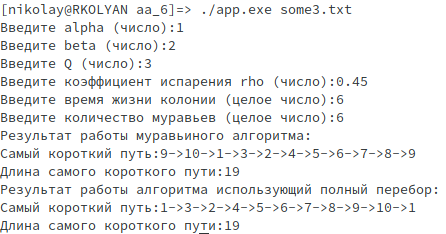
\includegraphics[scale=0.75]{example1.png}}
%\caption{Пример работы приложения}
%\label{images:example1}
%\end{figure}
%\begin{figure}[h]
%\center{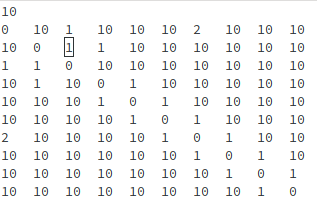
\includegraphics[scale=0.9]{example2.png}}
%\caption{Содержимое файла some3.txt}
%\label{images:example2}
%\end{figure}

\newpage
\subsection{Оценка времени выполнения}
%TODO
%\begin{figure}[h]
%\center{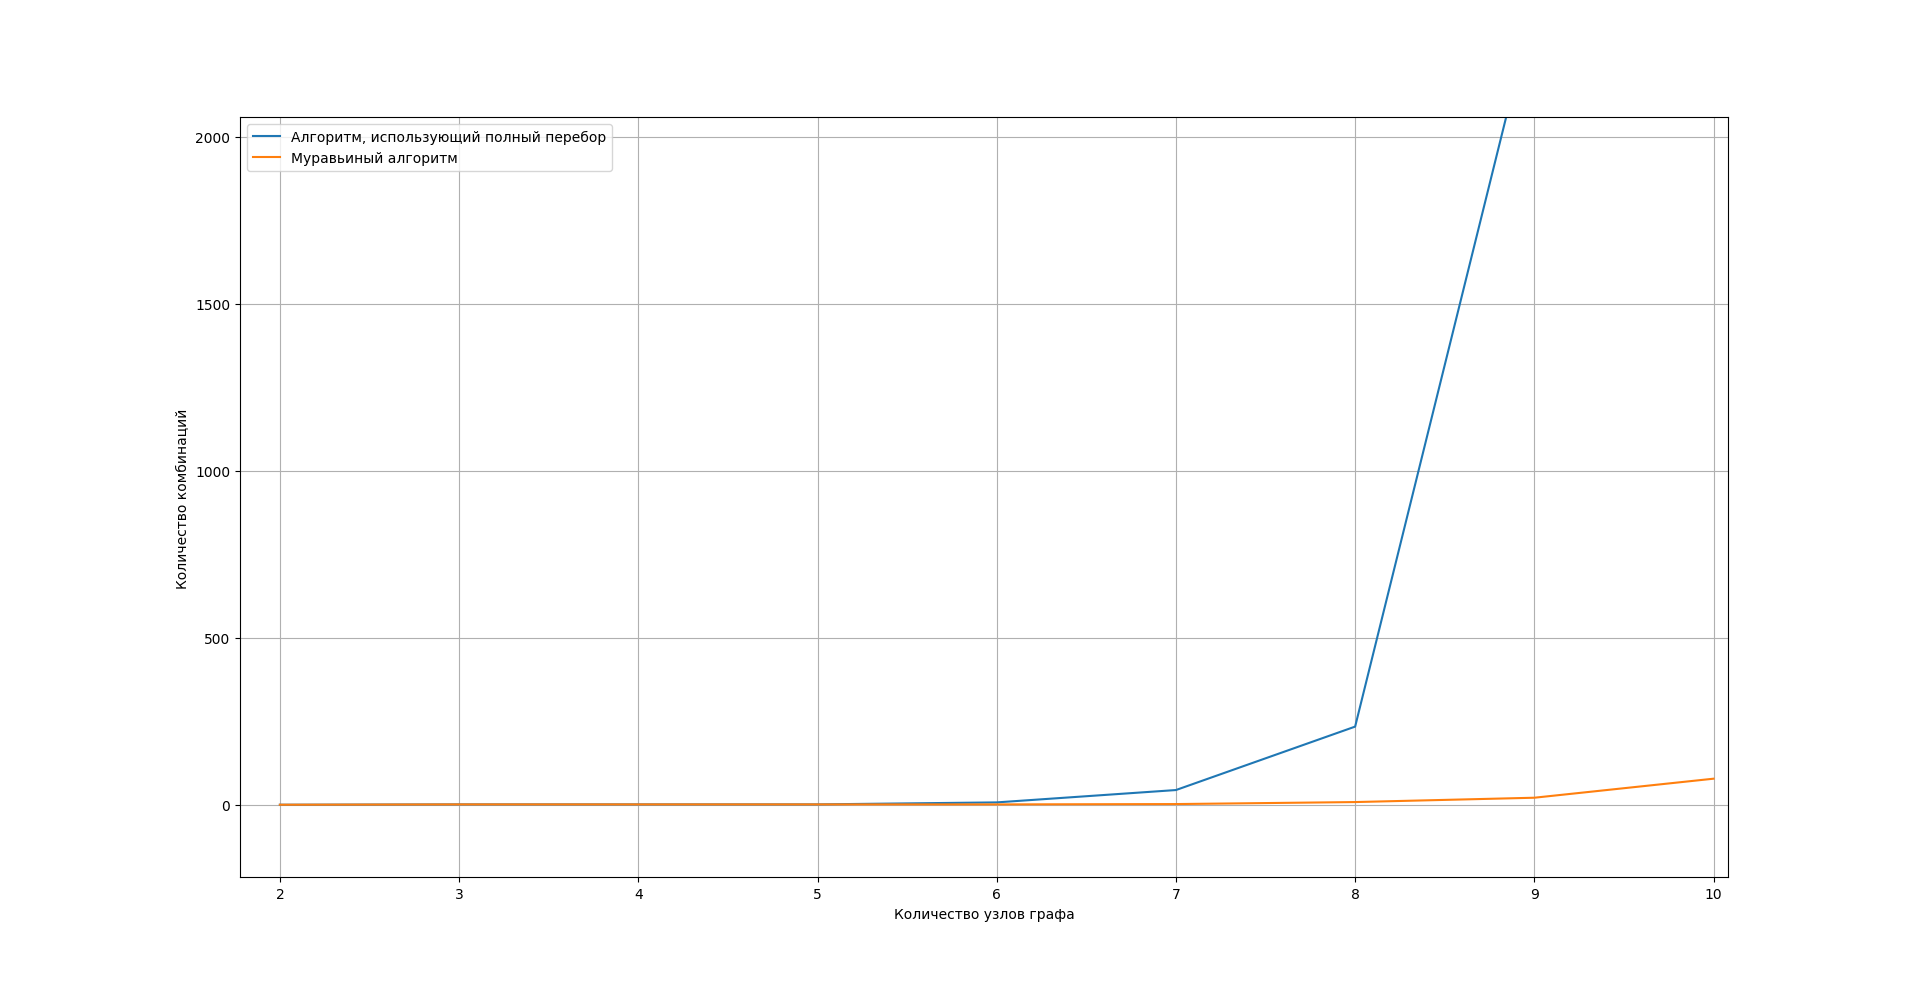
\includegraphics[scale=0.3]{graphics.png}}
%\caption{График}
%\label{graphics:graphic1}
%\end{figure}

\newpage
\subsection{Вывод}
Исходя из данных, полученных в результате эксперимента, можно сделать вывод, что муравьиный алгоритм значительно выигрывает у алгоритма, использующий метод полного перебора. При большом количестве узлов графа (как показано на графиках), алгоритм полного перебора \textbf{значительно} неэффективен. 

\newpage
\anonsection{ЗАКЛЮЧЕНИЕ}
Данные алгоритмы могут быть использованы не только как алгоритмы решения задачи коммивояжёра, но и как алгоритмы нахождения кратчайшего расстояния между двумя вершинами графа. Например, искать текущий минимальный маршрут между двумя городами имея определенную сеть дорог.
Муравьиный алгоритм (вернее, его модификации) на сегодняшний день признан одним из самых эффективных алгоритмов, решающих различные транспортные проблемы (пробки в городах, отсутствие прямого пути между пунктами назаначения и тд...).

\newpage
\anonsection{СПИСОК ИСТОЧНИКОВ}
\begin{enumerate}
\item Штовба С. Д. Муравьиные алгоритмы, Exponenta Pro. Математика в приложениях. 2004. № 4
\item Хабр, муравьиные алгоритмы - \url{https://habr.com/ru/post/105302/}
\end{enumerate}
\nocite{*}
\bibliographystyle{utf8gost705u}
\bibliography{biblio}

\end{document}
